\chapter{Results}
\label{chap4}

All tests, for CPU and GPU, had been run on the same device, Jetson Nano, the one provided from the course, and all 
results obtained are related to this hardware.

\section{Execution}

Before to run each execution be sure to compile using the available \emph{Makefile}.

To start execution it is possible run one of the bash scripts available.

\begin{itemize}
    \item \emph{run.sh}, to run all the GPU version.
    \item \emph{run\_CPU.sh}, to run all the CPU versions.
    \item \emph{run\_long.sh}, to run a long execution of a particular DFG using the version 4.1,
    the only that can carry such workload.
\end{itemize}

To run a single version directly three element are needed.

\begin{itemize}
    \item A file containing the DFG information, this file are obtained through original DFG file saved in .dot format.
    The conversion is achieved through a python script explained in appendix \ref{appendix1}.
    \item The value of area constrained.
    \item A file containing the all possible resources available. It is organized in the following way:
    \begin{itemize}
        \item first row is the number of operations k;
        \item then there are k rows containing the pair operation number and number n, representing the different resources;
        \item after each of these rows there are n row containing the pair area and speed of each resource that can execute that operation.
    \end{itemize}
\end{itemize}

The executable can be lunched in the following way:

\begin{lstlisting}
    dfg.o <dfg_name>.txt <RTL_file>.txt <area_constrained>
\end{lstlisting}

All latency, according DFG, are available inside a log file.

\section{Comparison}

In the following graphs, obtained from python script \emph{elaborate\_data.py} (appendix \ref{appendix2}),
it is possible to observe the performances of the all versions using different DFG and area constraint.
A lot of other tests had been run to check not only performances but also the correctness of the scheduling
but the ones show here are the most significant.
It's important to notice that version 1 is useless because, when it works, all versions, GPU and CPU,
have time execution almost equal to zero second.

\begin{figure}[!h]
    \centering
    \begin{subfigure}{.45\textwidth}
        \centering
        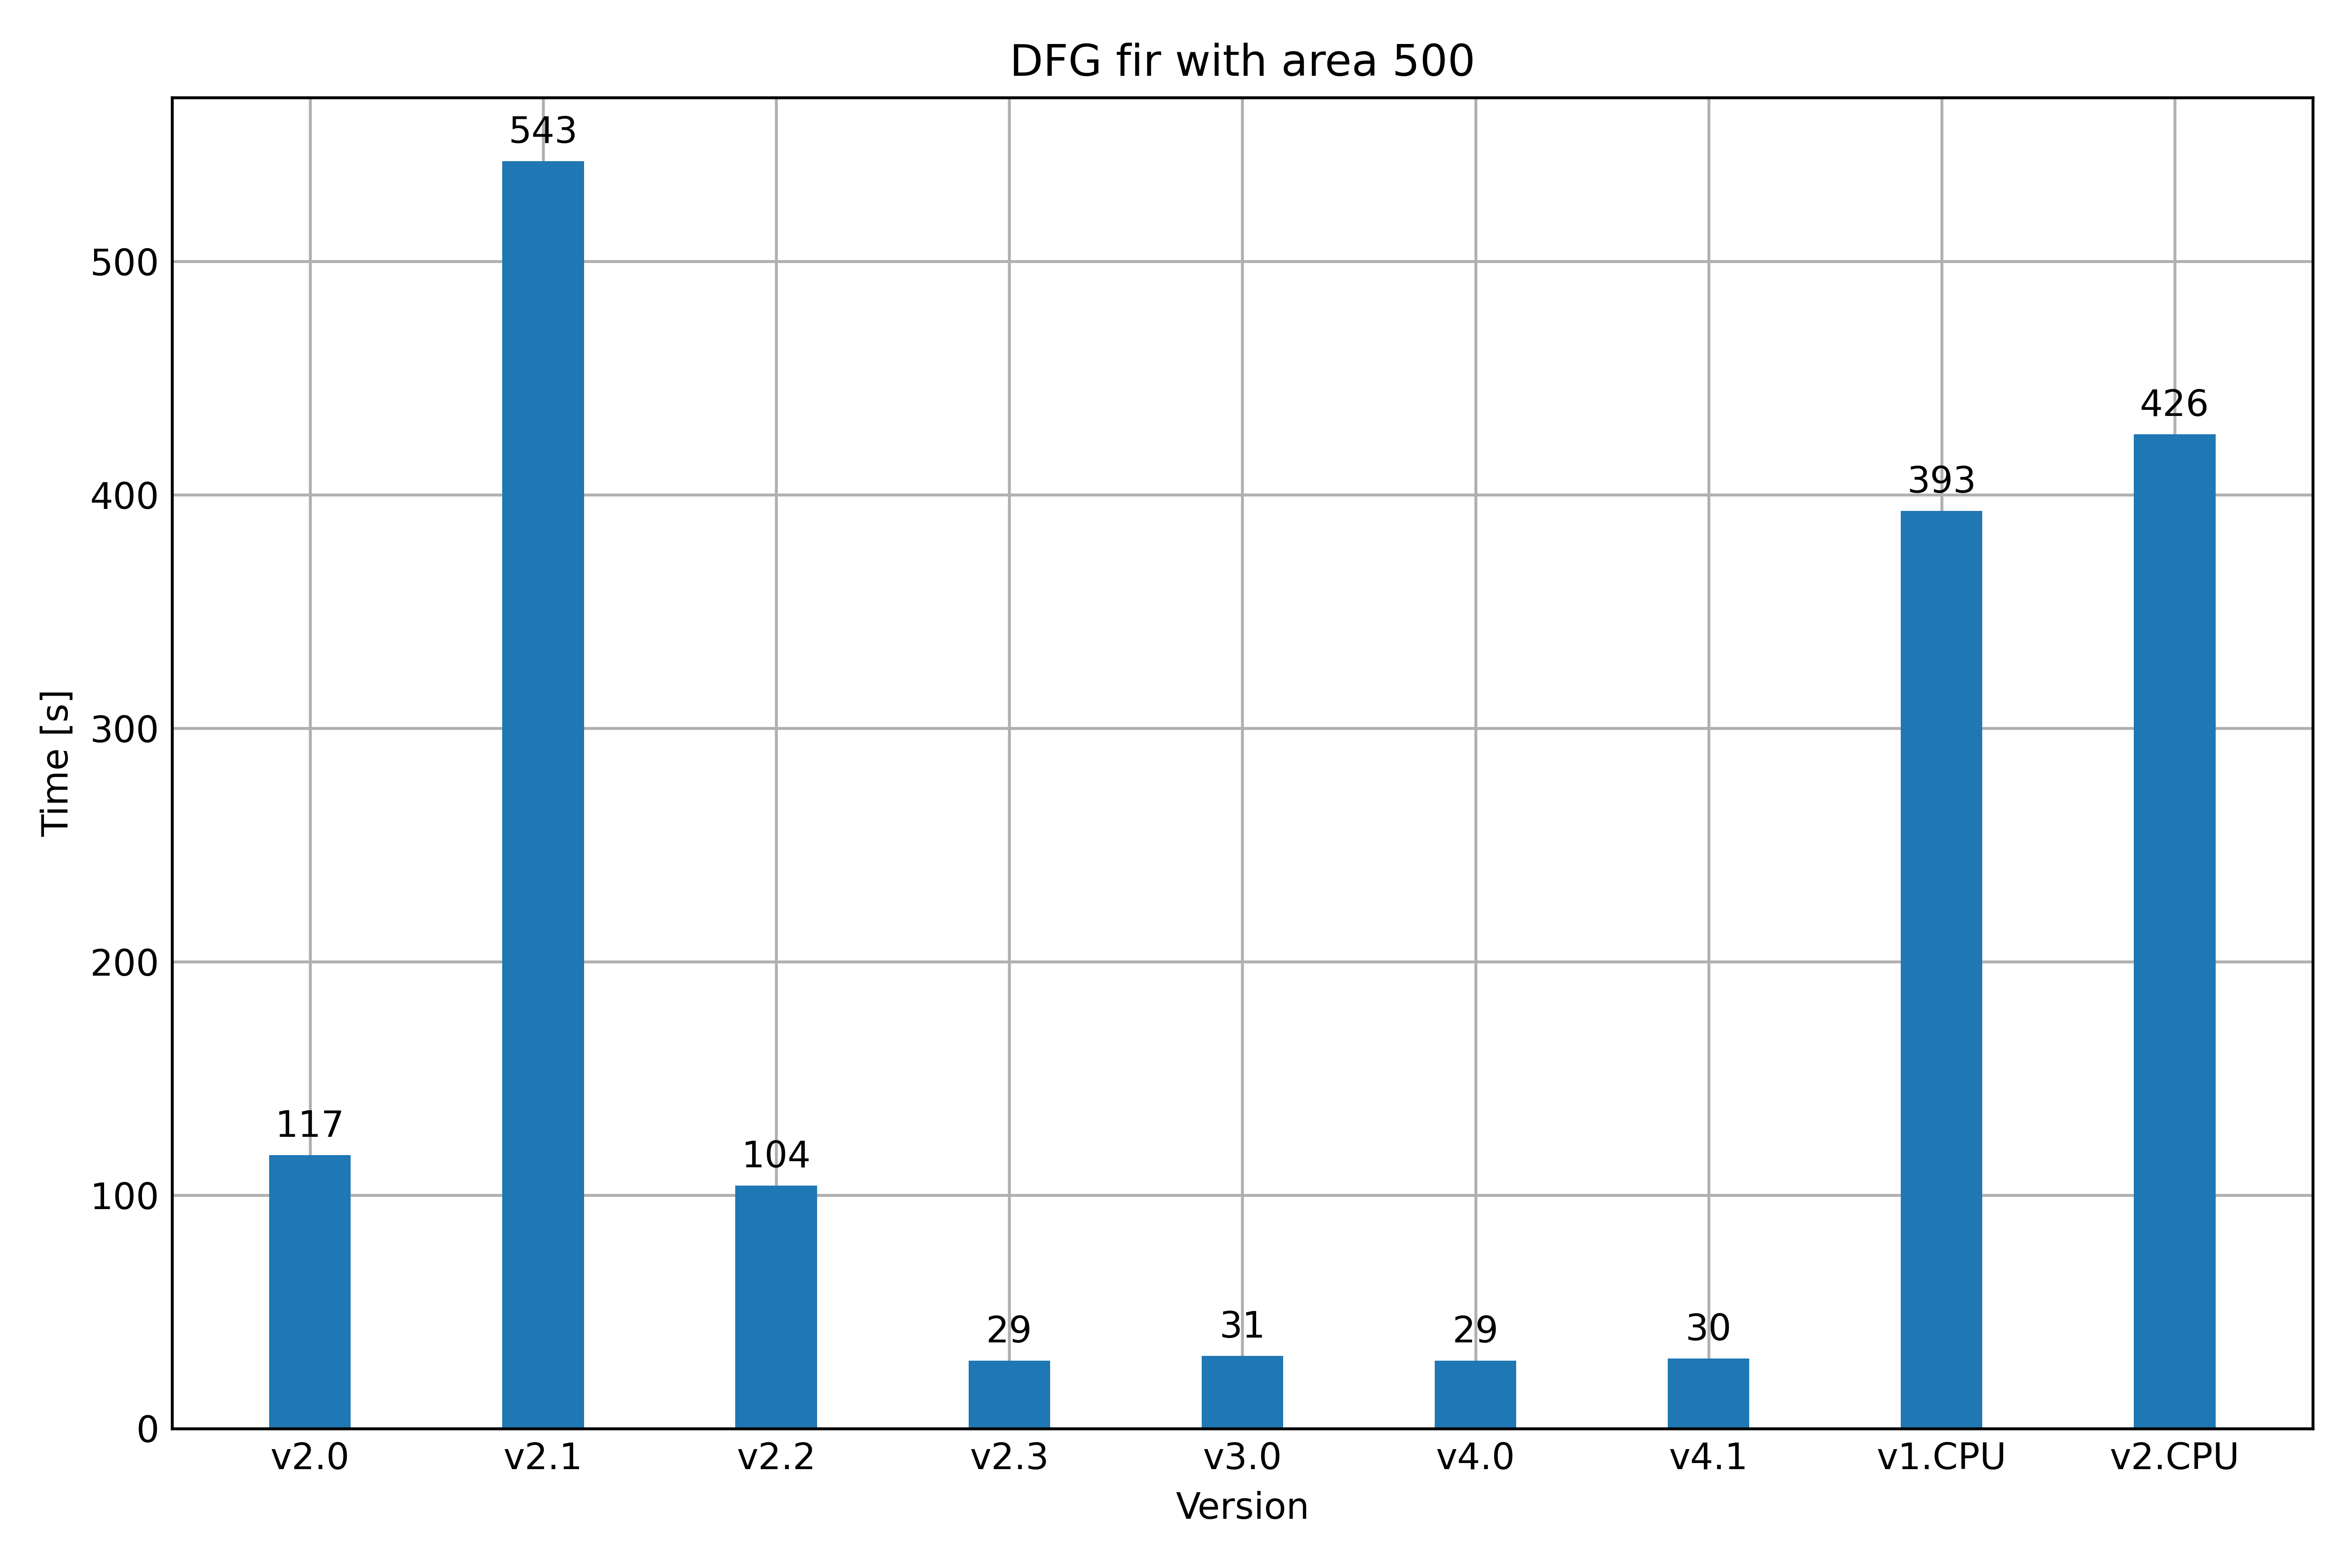
\includegraphics[width=.95\linewidth]{chapters/figures/fir_500.png}  
        \caption{fir bar graph with area 500}
        \label{fig:fir_500}
    \end{subfigure}
    \begin{subfigure}{.45\textwidth}
        \centering
        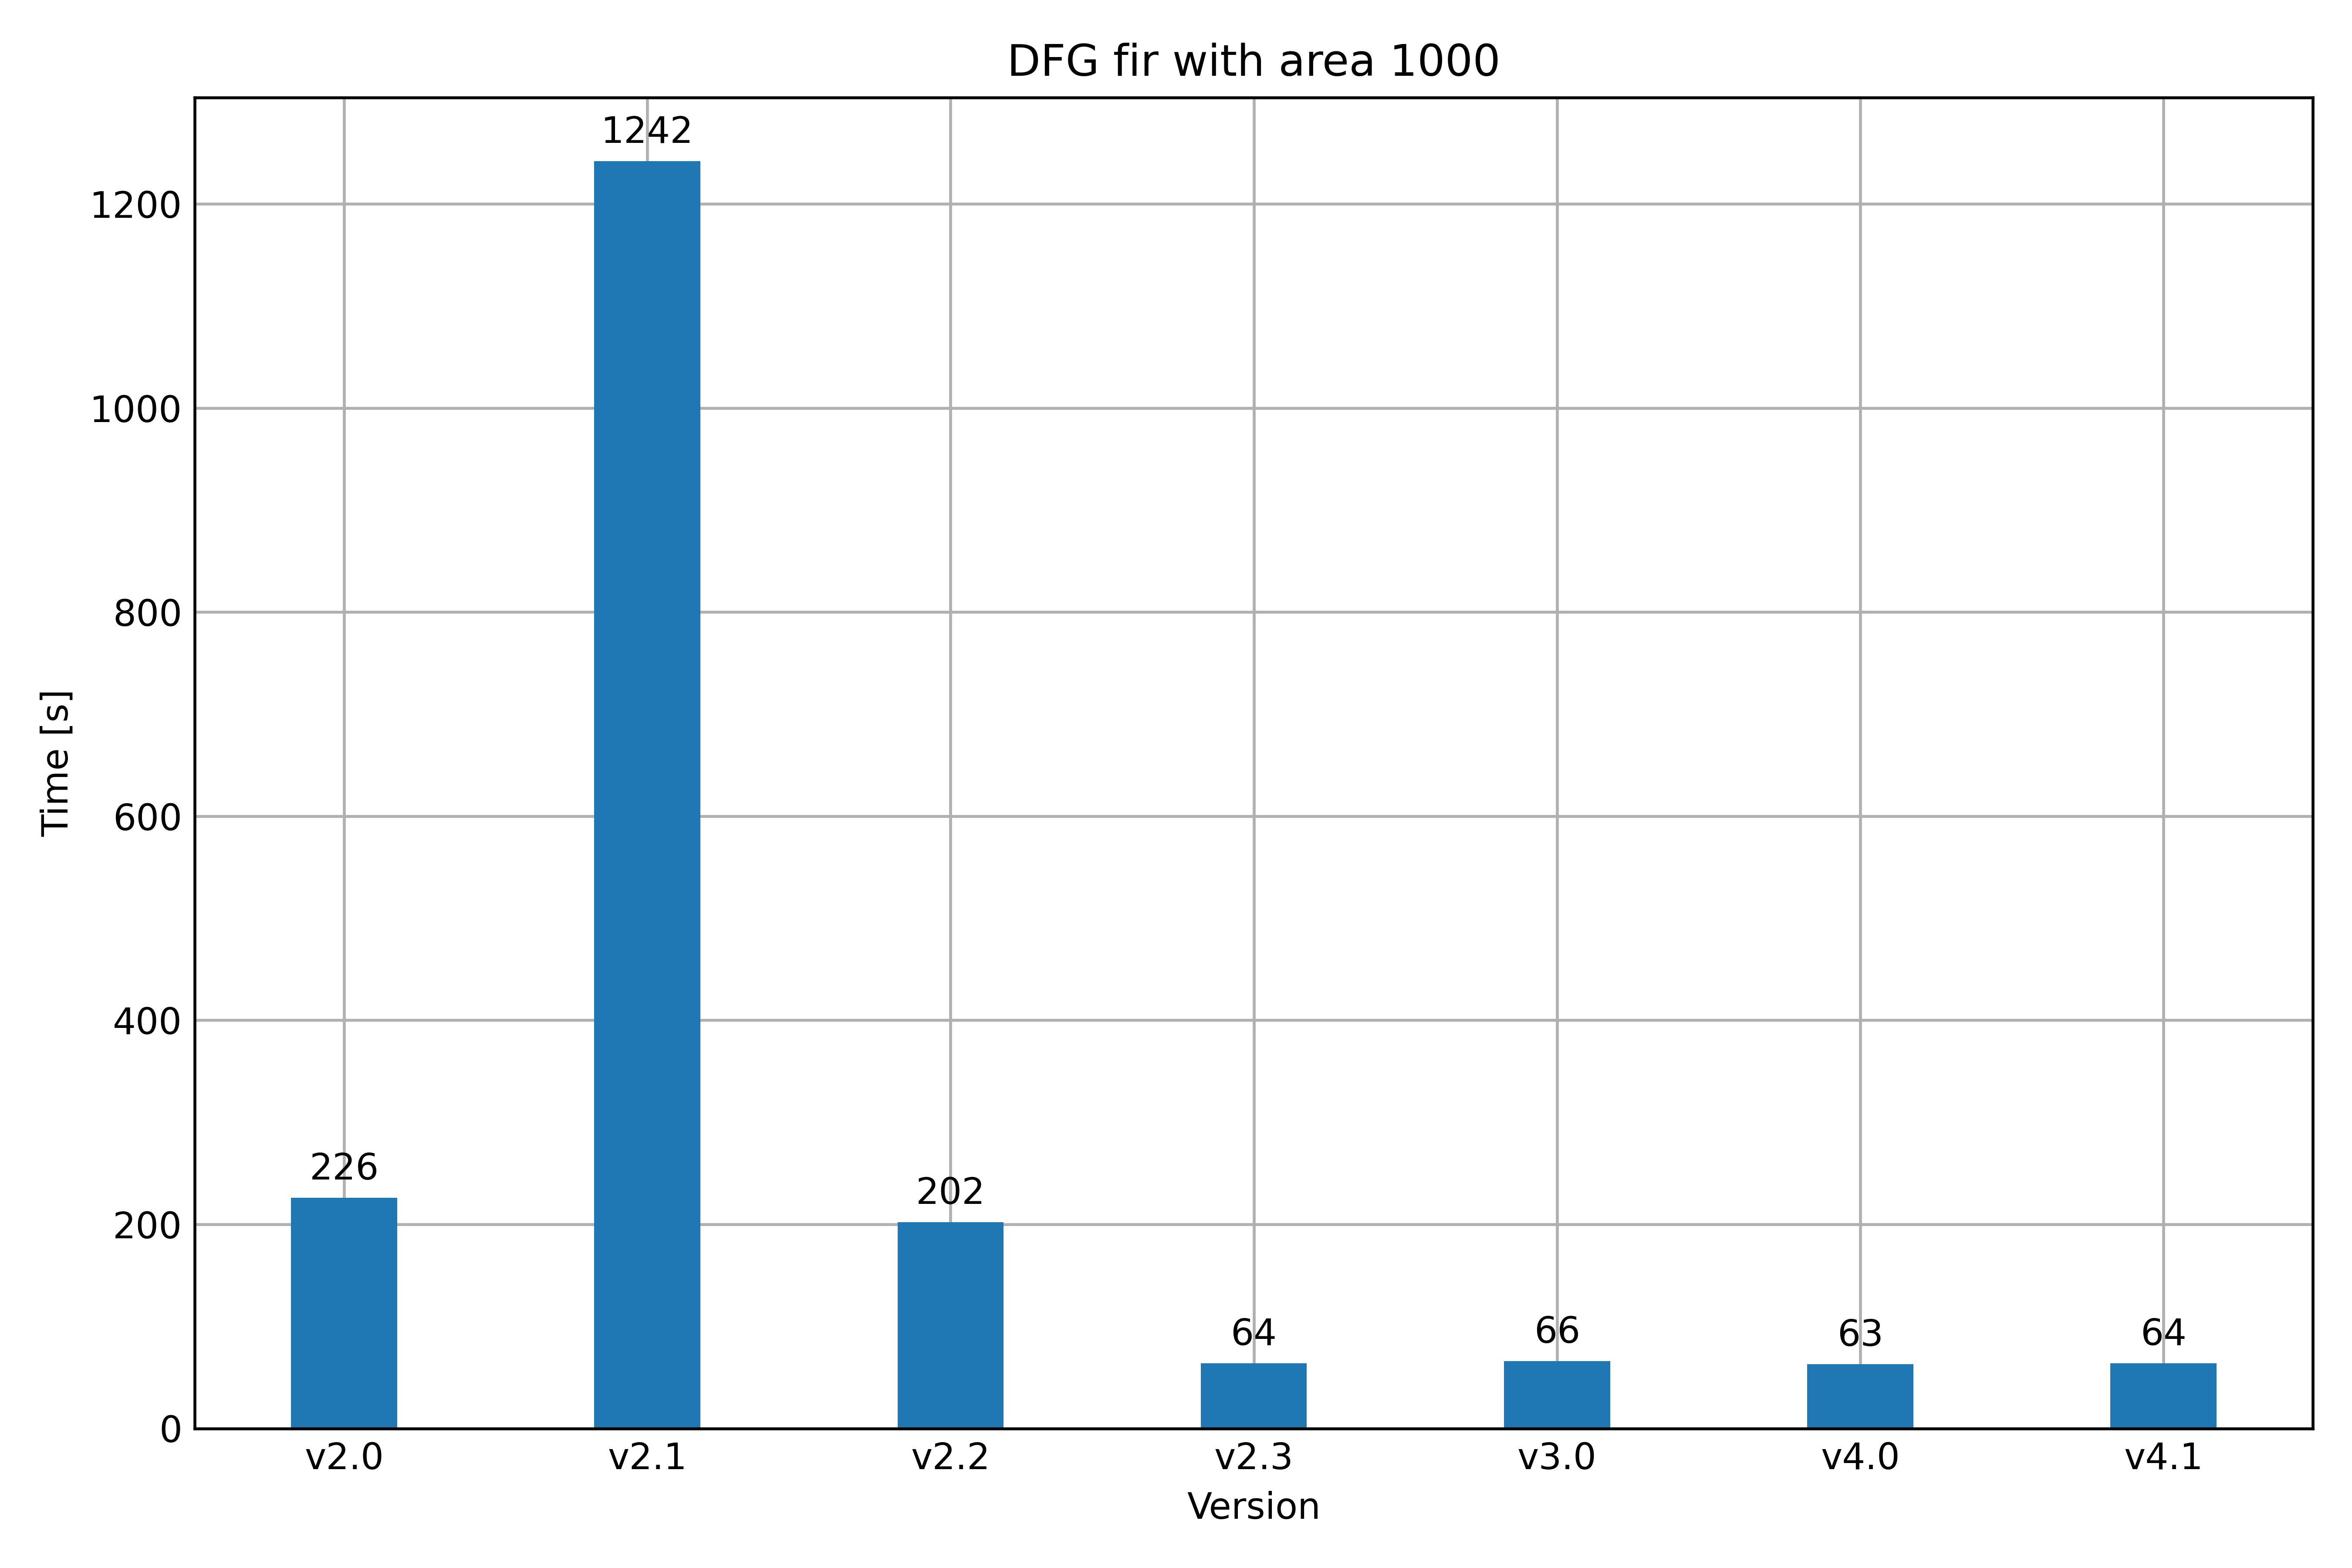
\includegraphics[width=.95\linewidth]{chapters/figures/fir_1000.png}  
        \caption{fir bar graph with area 1000}
        \label{fig:fir_1000}
    \end{subfigure}
\end{figure}

\begin{figure}[h]
    \centering
    \begin{subfigure}{.45\textwidth}
        \centering
        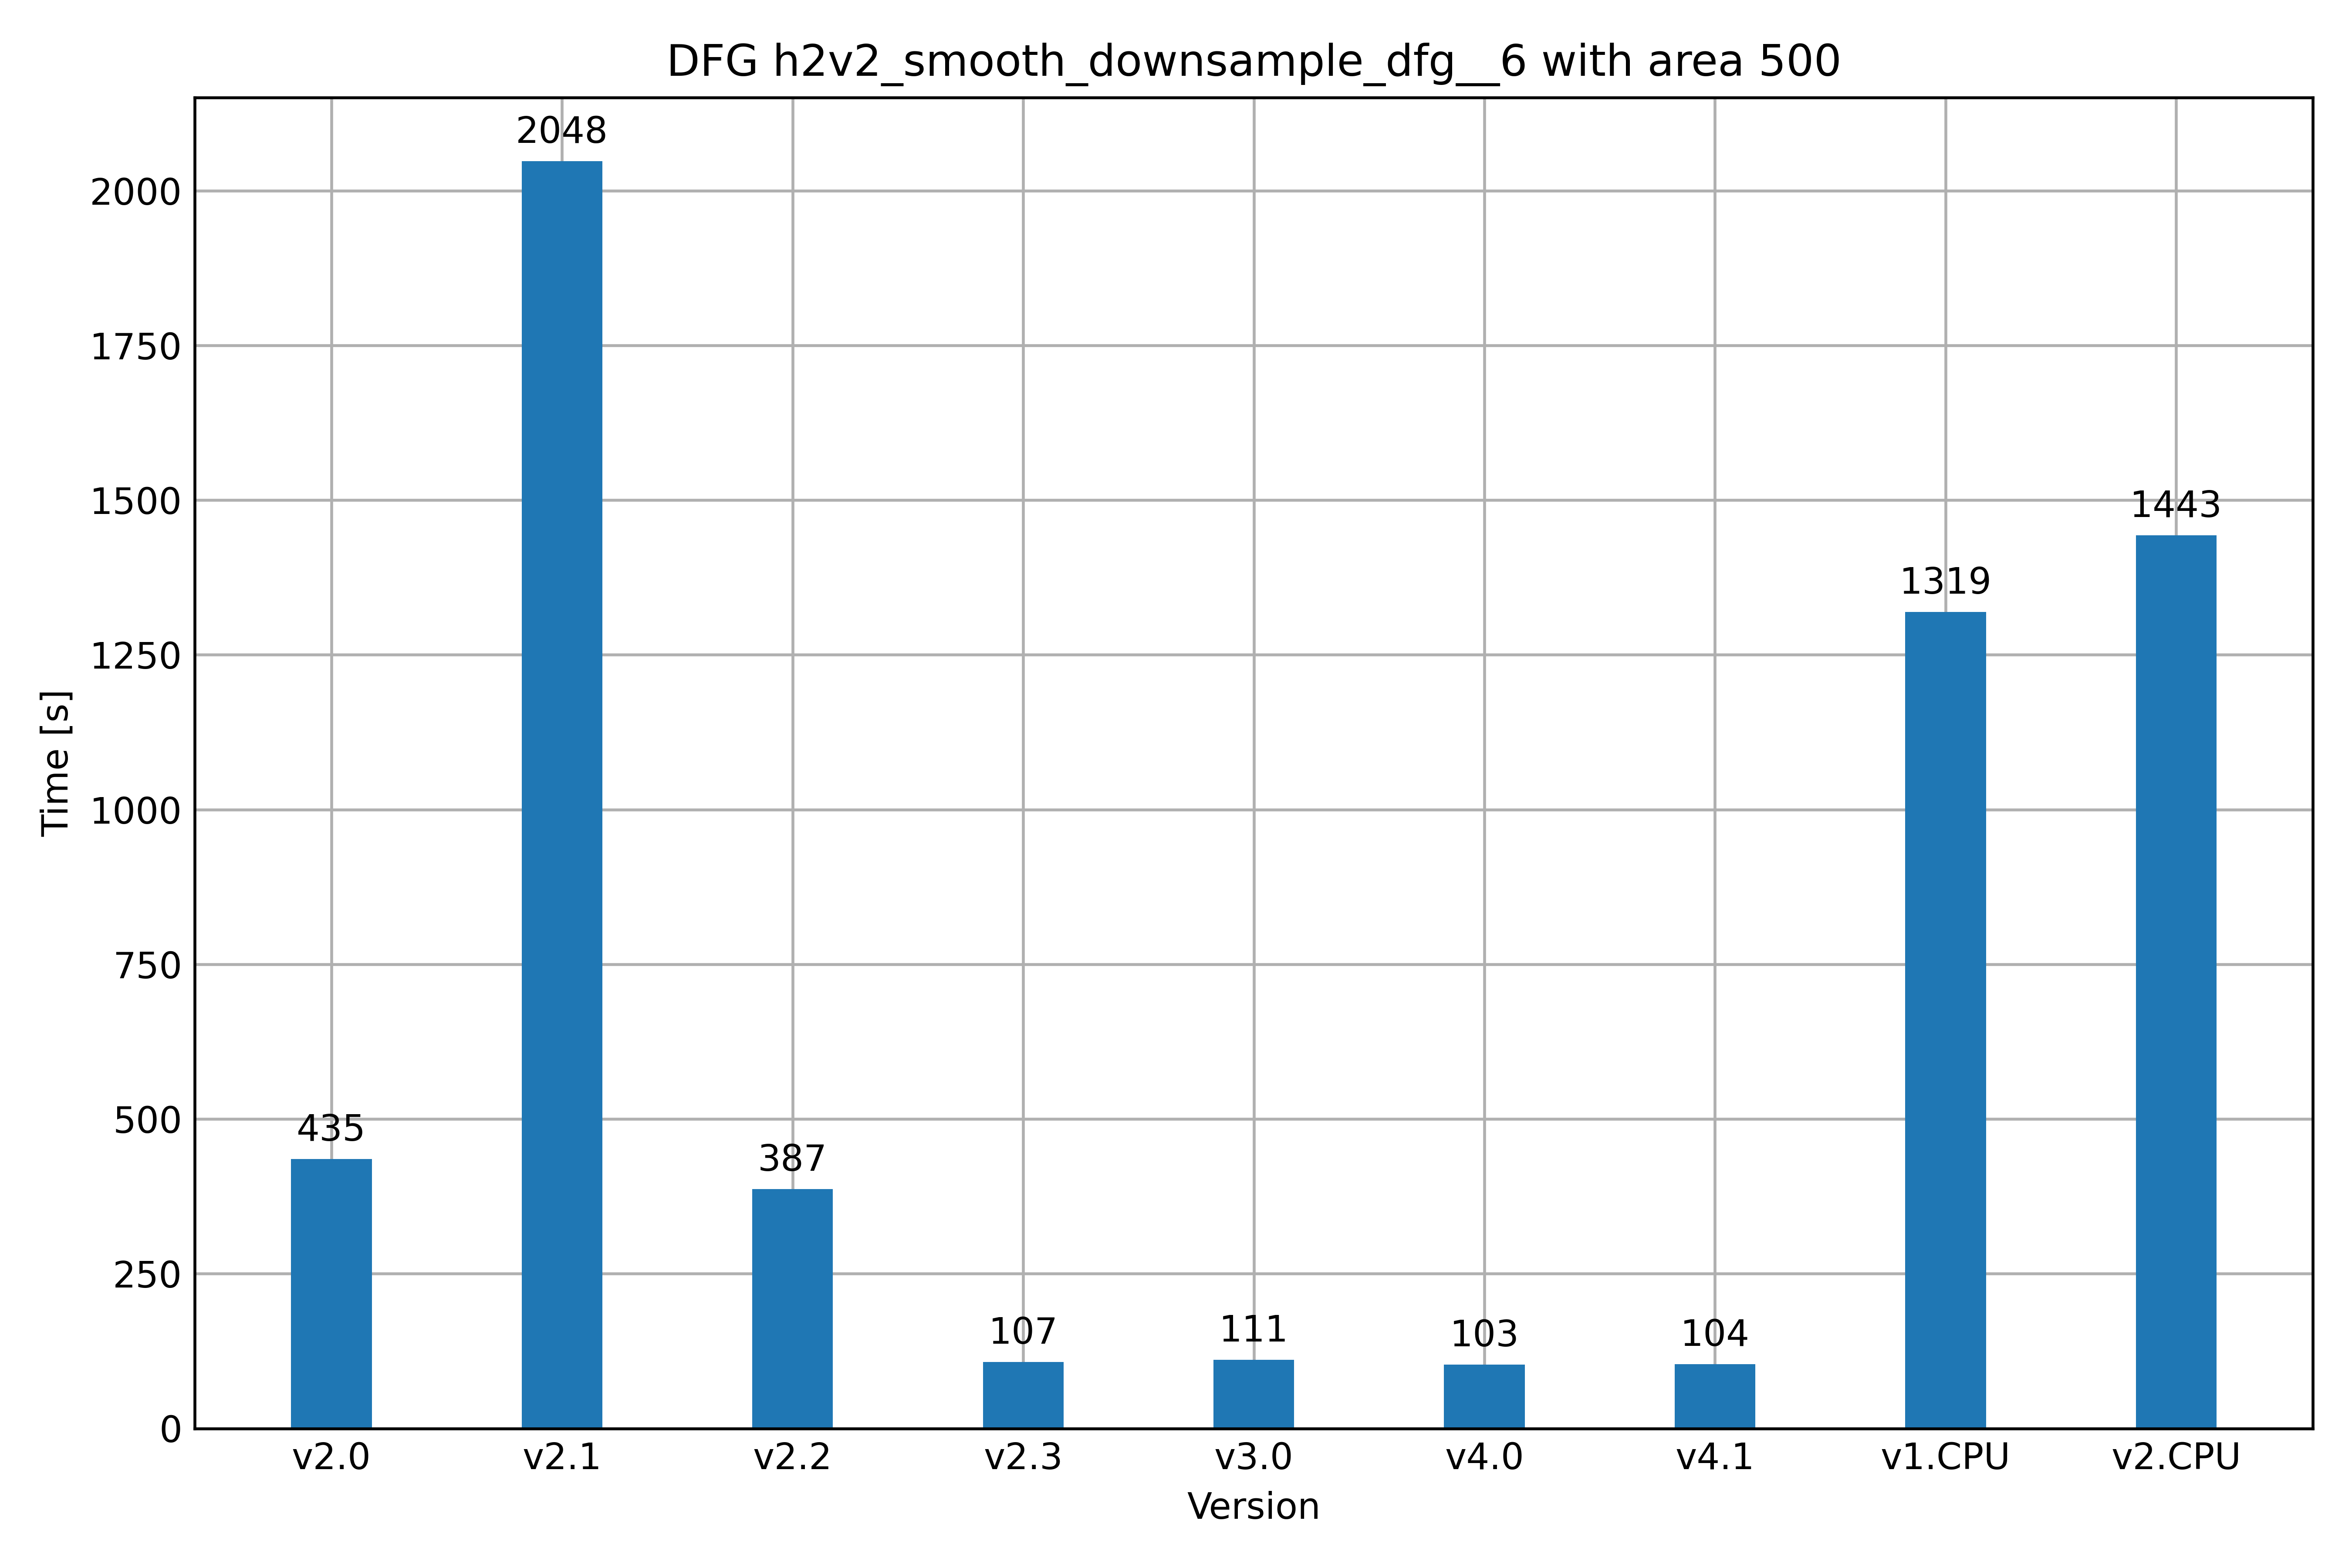
\includegraphics[width=.95\linewidth]{chapters/figures/h2v2_smooth_downsample_dfg__6_500.png}  
        \caption{h2v2 with area 500 bar graph}
        \label{fig:h2v2_500}
    \end{subfigure}
    \begin{subfigure}{.45\textwidth}
        \centering
        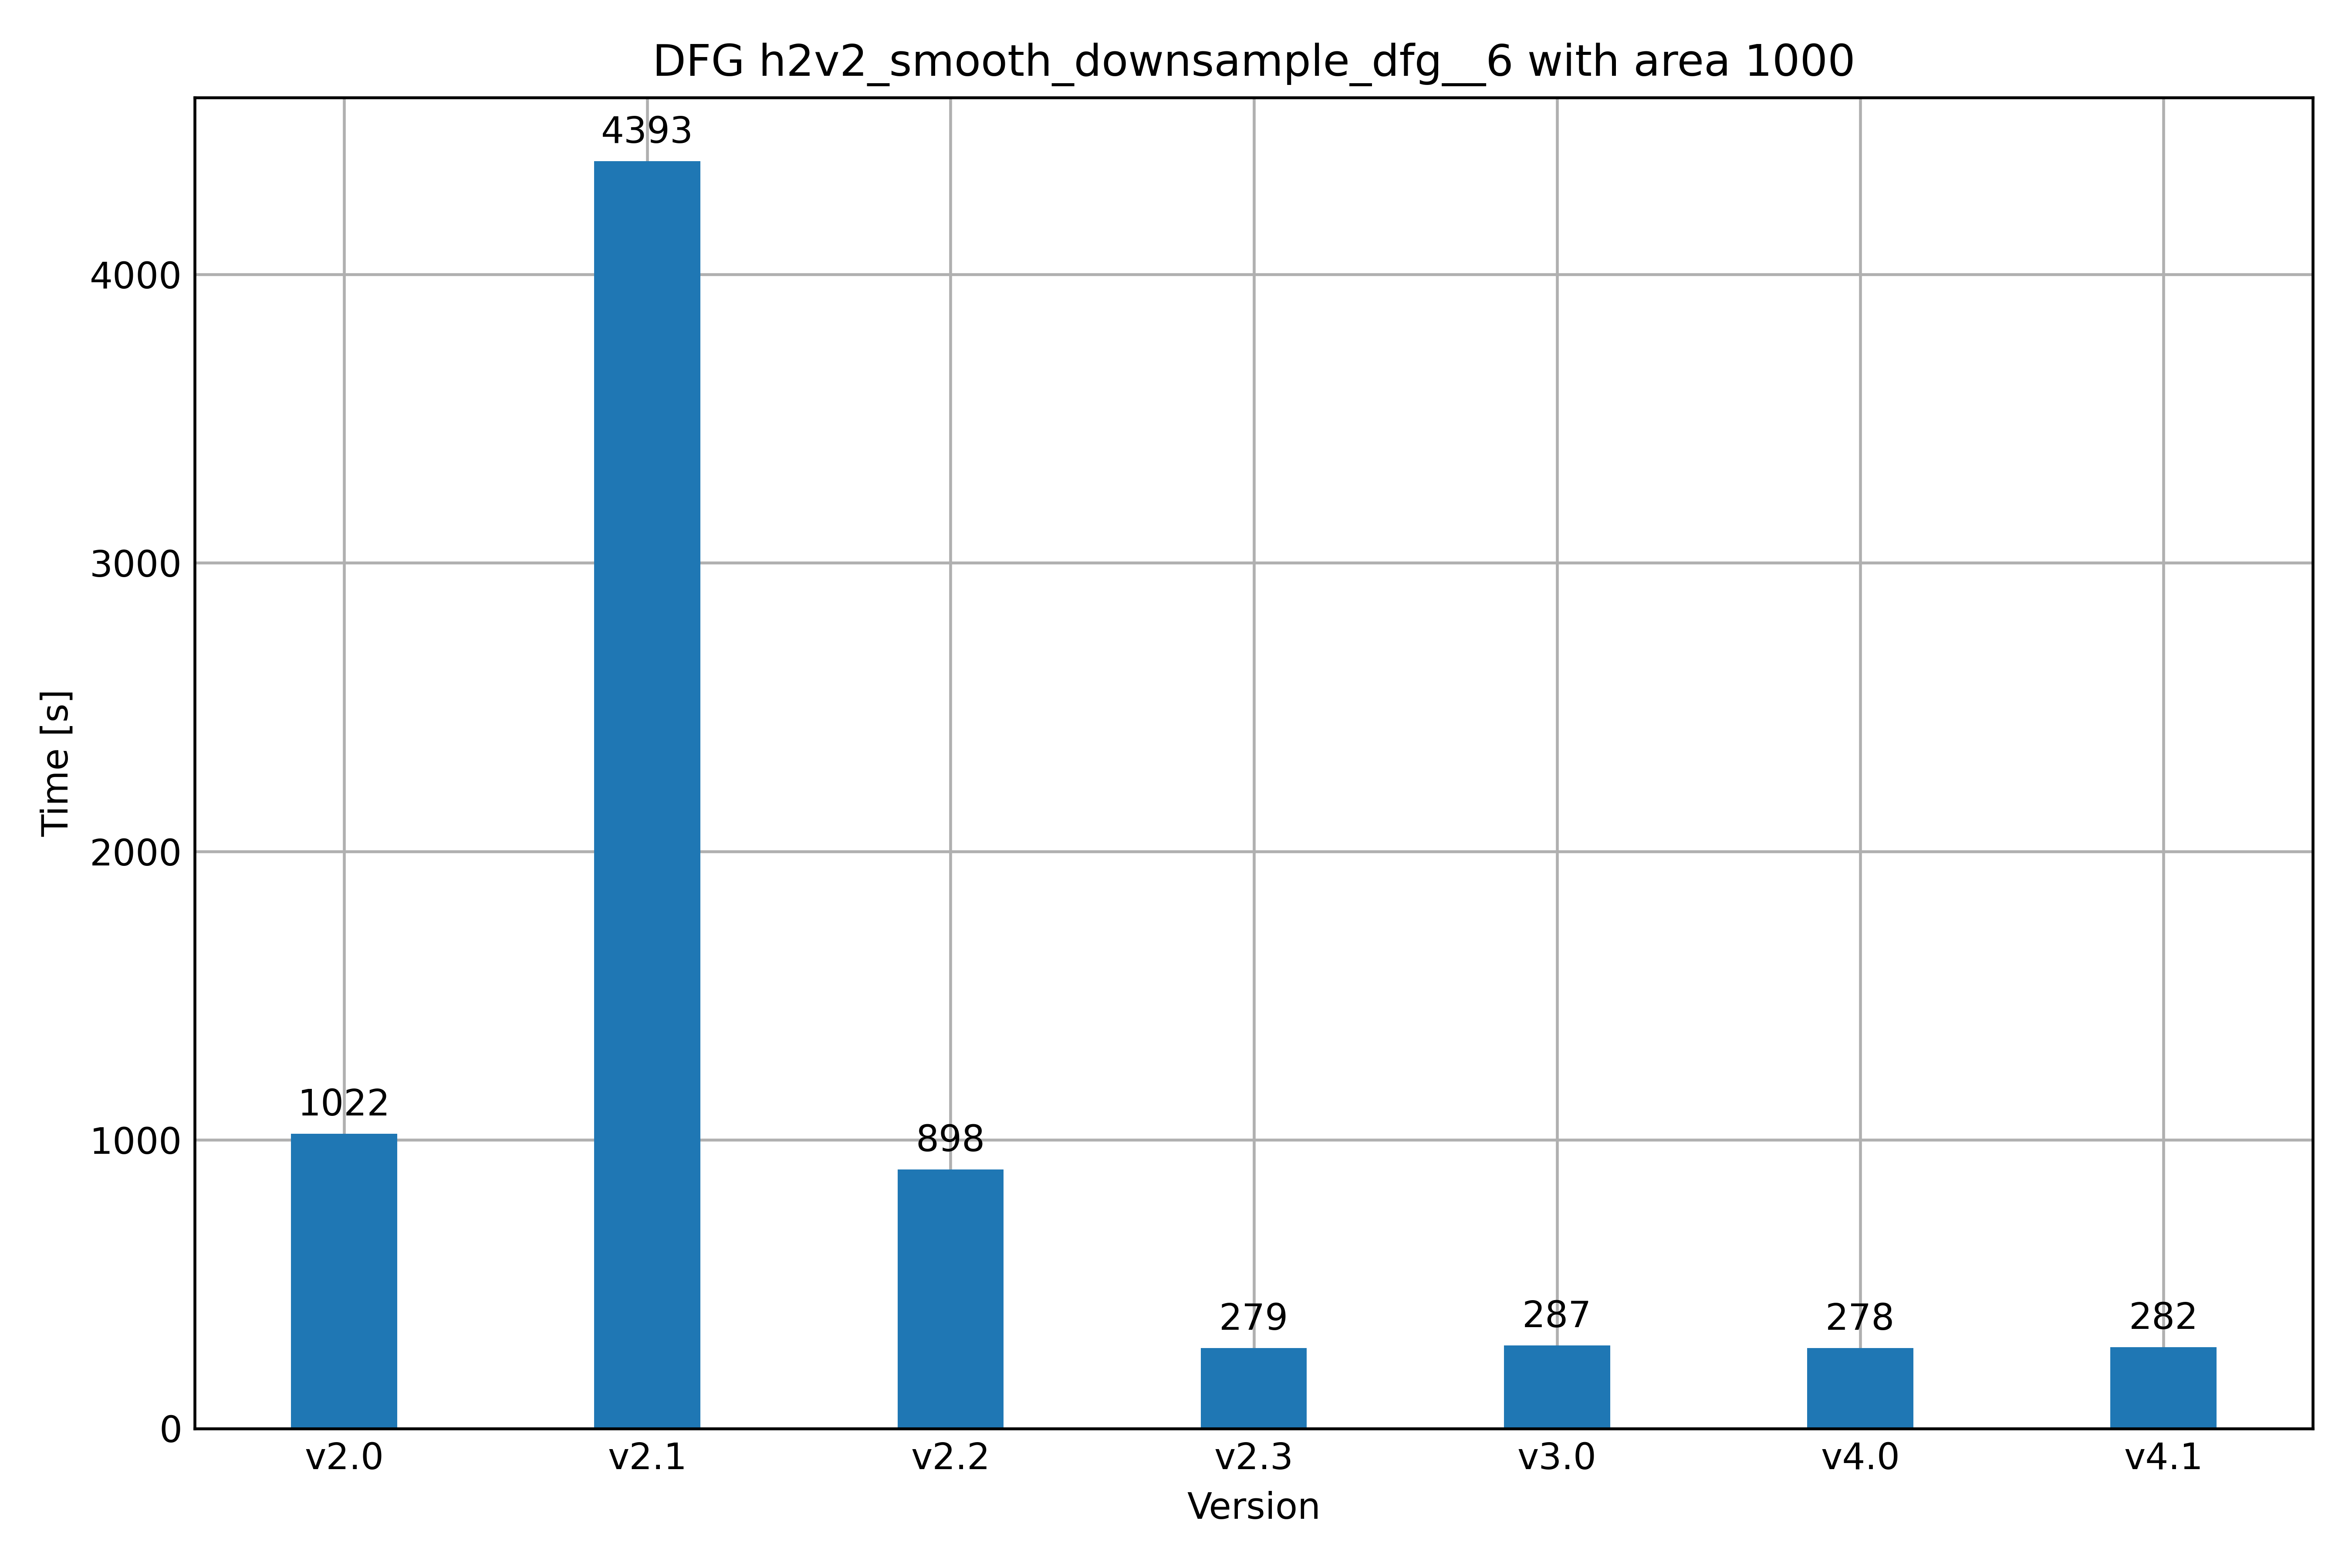
\includegraphics[width=.95\linewidth]{chapters/figures/h2v2_smooth_downsample_dfg__6_1000.png}  
        \caption{h2v2 with area 1000 bar graph}
        \label{fig:h2v2_1000}
    \end{subfigure}
\end{figure}

In the figure \ref{fig:fir_500} and \ref{fig:h2v2_500} it's possible to appreciate the advantage to exploit GPU.
Beside the version 2.1 spent the greatest time, all the others have significant improvement in time, 
also respect to the first basic version 2.0 and 2.3.

Version 2.3, 3.0 and 4.0 have almost the same result, also if 4.0 produces always the best ones. This could be due to 
the virtualization process employed from GPU that, on Jetson Nano, it's quite limited or due to the Operating System internal 
scheduling.

More precise data are available in repository, under \emph{result} folder.

\section{Conclusion}

The code running on GPU respect to the CPU is speed up of 14 times, that is an important quantity.

Like premeditated in chapter \ref{chap3} then last version is the best one. Using the internal registers inside GPU,
the fastest memory type, and using much more blocks inside each stream, has been possible the reach the best performance.

Streams have been important:
\begin{itemize}
    \item they allowed to have a further grade of parallelization of the workload;
    \item they allowed to use asynchronous copy of global memory, much faster than synchronous version, of course this operation 
    have been limitated as much as possible like explained in the above chapters.
\end{itemize}

The final version take care of all possible workload problems is the 4.1 that, cause to this little overhead,
is a little heavier than the 4.0. All the other final version, like 2.3 and 3.0, don't look to have a big 
differences in percentage improvement but, on long execution time, important speed up could be achieved in 4.0 and
the versions 4.1 could be used to handle huge quantity of threads.
